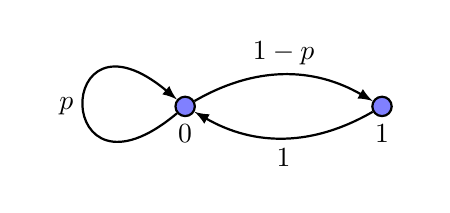
\begin{tikzpicture}[>=latex]
    \clip (-2, -1) rectangle (3, 1);
    
    \tikzstyle{vert} = [circle, draw, thick, fill = blue!50, inner sep = 0pt, minimum size = 7pt]

    \node[vert] (a) at (0, 0) {};
    \node[below = 3pt] at (a) {$0$};

    \node[vert] (b) at (2.5, 0) {};
    \node[below = 3pt] at (b) {$1$};

    \draw[->, thick] (a) to[out = 220, in = 140, loop, looseness = 30]
        node[midway, left, black] {$p$} (a);  
    \draw[->, thick] (a) to[bend left] node[midway, above, black] {$1 - p$} (b);
    \draw[->, thick] (b) to[bend left] node[midway, below, black] {$1$} (a);
\end{tikzpicture}